\problemname{Gratis mat}

Hsara älskar gratis mat.

Ikväll är Hsara på restaurang med jobbet, och Hsara sitter och analyserar möjligheterna för att få middagen betald. Precis en person kommer att betala för hela middagen (allas mat), men inte vilken person som helst. Det är endast tillåtet att betala för middagen om ingen överordnad (eventuellt indirekt, t.ex. din chefs chef) i organisationen befinner sig vid bordet.

Organisationen består av $N$ personer numrerade från $1$ till $N$. Varje person, förutom organisationens VD, har exakt en chef. Givet varje persons chef och en lista över personer som är närvarande vid bordet, avgör hur många som skulle kunna betala för middagen.

\begin{figure}[h!]
	\begin{center}
		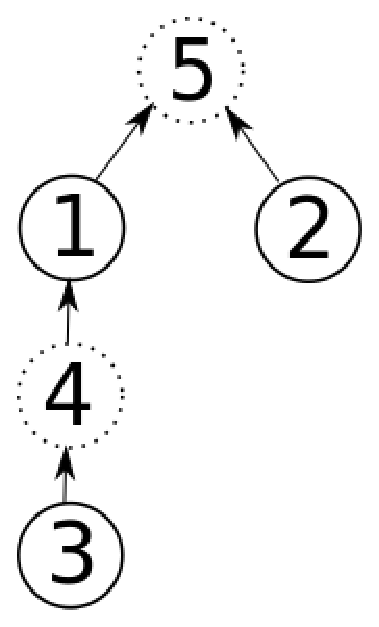
\includegraphics[width=0.2\textwidth]{tree.eps}
		\caption{Illustration av hur organisationen i det första exemplet ser ut.}
	\end{center}
\end{figure}

\section*{Input}

Den första raden i indatan innehåller två heltal, $N$ - antalet personer i organisationen och $M$ - antalet personer vid bordet.

Den andra raden innehåller $N$ heltal. Det $i$:te talet anger vem som är chef till person $i$. 0 innebär att personen inte har en chef och därmed är VD för organisationen. Det finns precis en person som är VD.

Den tredje raden innehåller $M$ heltal ($1 \le M \le N$) som anger vilka som sitter vid bordet.

\section*{Output}
Skriv ut ett heltal - antalet personer vid bordet som skulle kunna betala för middagen.

\section*{Poängsättning}
Din lösning kommer att testas på en mängd testfallsgrupper. För att få poäng för en grupp så måste du klara alla testfall i gruppen.

\begin{tabular}{| l | l | l |}
	\hline
	Grupp & Poängvärde & Begränsningar\\ \hline
  1     & 49         & $2 \le N \le 2\,000$ \\ \hline
  2     & 51         & $2 \le N \le 100\,000$. \\ \hline
\end{tabular}

\section*{Förklaring}
I det första exemplet kan personerna 1 och 2 betala. Person 3 kan inte betala eftersom person 1 sitter vid bordet.

I det andra exemplet är person 5 VD och sitter vid bordet. Därför kan bara person 5 betala.
